% Created by tikzDevice version 0.12.6 on 2026-08-08 13:32:30
% !TEX encoding = UTF-8 Unicode
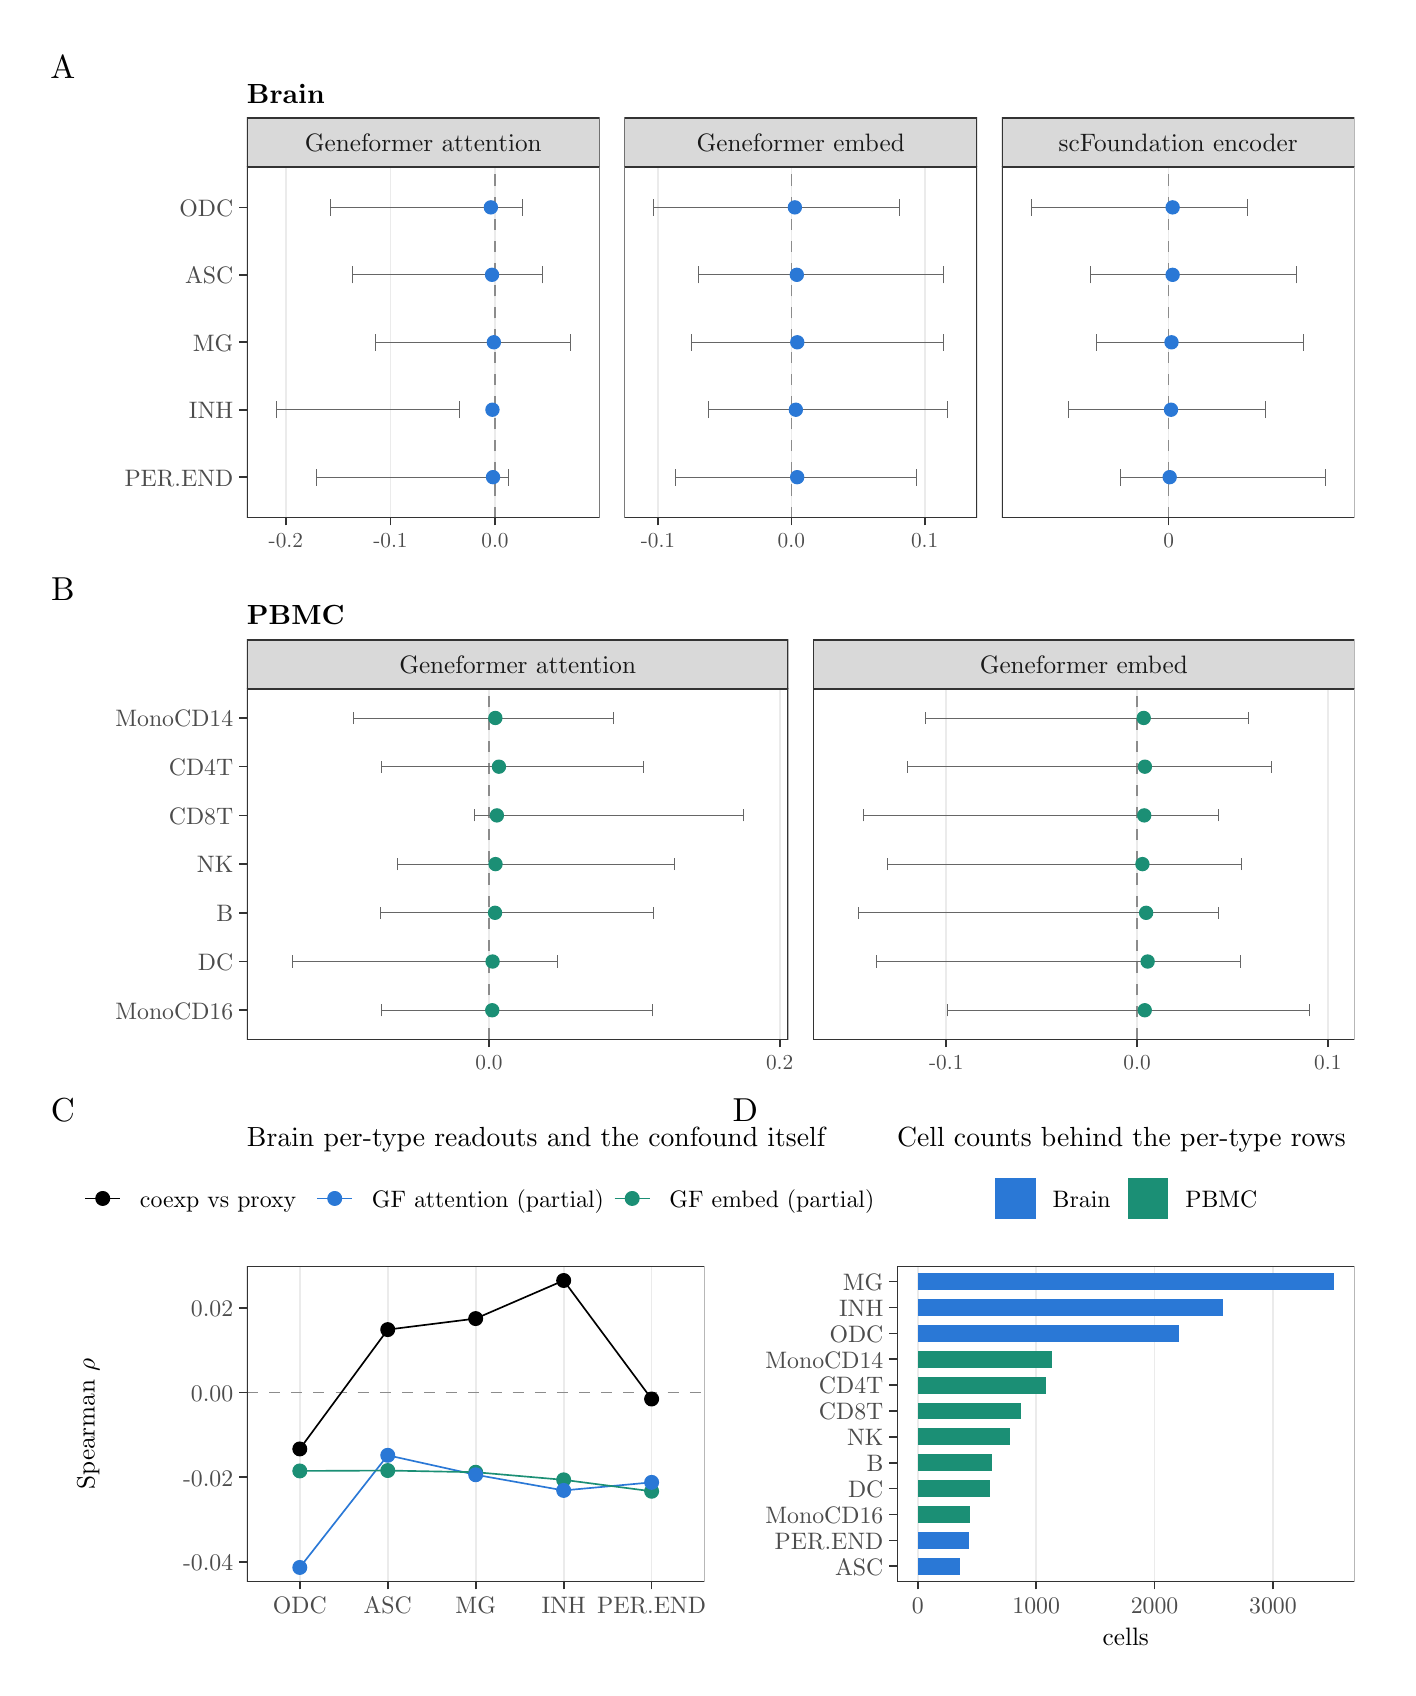
\begin{tikzpicture}[x=1pt,y=1pt]
\definecolor{fillColor}{RGB}{255,255,255}
\path[use as bounding box,fill=fillColor,fill opacity=0.00] (0,0) rectangle (491.44,592.61);
\begin{scope}
\path[clip] (  0.00,  0.00) rectangle (491.44,592.61);
\definecolor{drawColor}{RGB}{255,255,255}
\definecolor{fillColor}{RGB}{255,255,255}

\path[draw=drawColor,line width= 0.6pt,line join=round,line cap=round,fill=fillColor] ( -0.00, -0.00) rectangle (491.44,592.61);
\end{scope}
\begin{scope}
\path[clip] (  4.00,400.05) rectangle (485.44,588.61);
\definecolor{drawColor}{RGB}{255,255,255}
\definecolor{fillColor}{RGB}{255,255,255}

\path[draw=drawColor,line width= 0.6pt,line join=round,line cap=round,fill=fillColor] (  4.00,400.05) rectangle (485.44,588.61);
\end{scope}
\begin{scope}
\path[clip] (  4.00,211.49) rectangle (485.44,400.05);
\definecolor{drawColor}{RGB}{255,255,255}
\definecolor{fillColor}{RGB}{255,255,255}

\path[draw=drawColor,line width= 0.6pt,line join=round,line cap=round,fill=fillColor] (  4.00,211.49) rectangle (485.44,400.05);
\end{scope}
\begin{scope}
\path[clip] ( 79.25,415.55) rectangle (206.65,542.29);
\definecolor{fillColor}{RGB}{255,255,255}

\path[fill=fillColor] ( 79.25,415.55) rectangle (206.65,542.29);
\definecolor{drawColor}{gray}{0.92}

\path[draw=drawColor,line width= 0.6pt,line join=round] ( 93.31,415.55) --
	( 93.31,542.29);

\path[draw=drawColor,line width= 0.6pt,line join=round] (131.09,415.55) --
	(131.09,542.29);

\path[draw=drawColor,line width= 0.6pt,line join=round] (168.87,415.55) --
	(168.87,542.29);
\definecolor{drawColor}{gray}{0.55}

\path[draw=drawColor,line width= 0.6pt,dash pattern=on 4pt off 4pt ,line join=round] (168.87,415.55) -- (168.87,542.29);
\definecolor{drawColor}{gray}{0.40}

\path[draw=drawColor,line width= 0.3pt,line join=round] (178.73,524.62) --
	(178.73,530.72);

\path[draw=drawColor,line width= 0.3pt,line join=round] (178.73,527.67) --
	(109.55,527.67);

\path[draw=drawColor,line width= 0.3pt,line join=round] (109.55,524.62) --
	(109.55,530.72);

\path[draw=drawColor,line width= 0.3pt,line join=round] (185.87,500.25) --
	(185.87,506.34);

\path[draw=drawColor,line width= 0.3pt,line join=round] (185.87,503.30) --
	(117.41,503.30);

\path[draw=drawColor,line width= 0.3pt,line join=round] (117.41,500.25) --
	(117.41,506.34);

\path[draw=drawColor,line width= 0.3pt,line join=round] (196.03,475.88) --
	(196.03,481.97);

\path[draw=drawColor,line width= 0.3pt,line join=round] (196.03,478.92) --
	(125.69,478.92);

\path[draw=drawColor,line width= 0.3pt,line join=round] (125.69,475.88) --
	(125.69,481.97);

\path[draw=drawColor,line width= 0.3pt,line join=round] (156.06,451.50) --
	(156.06,457.60);

\path[draw=drawColor,line width= 0.3pt,line join=round] (156.06,454.55) --
	( 89.87,454.55);

\path[draw=drawColor,line width= 0.3pt,line join=round] ( 89.87,451.50) --
	( 89.87,457.60);

\path[draw=drawColor,line width= 0.3pt,line join=round] (173.55,427.13) --
	(173.55,433.22);

\path[draw=drawColor,line width= 0.3pt,line join=round] (173.55,430.18) --
	(104.19,430.18);

\path[draw=drawColor,line width= 0.3pt,line join=round] (104.19,427.13) --
	(104.19,433.22);
\definecolor{drawColor}{RGB}{42,120,214}
\definecolor{fillColor}{RGB}{42,120,214}

\path[draw=drawColor,line width= 0.4pt,line join=round,line cap=round,fill=fillColor] (167.37,527.67) circle (  2.39);

\path[draw=drawColor,line width= 0.4pt,line join=round,line cap=round,fill=fillColor] (167.80,503.30) circle (  2.39);

\path[draw=drawColor,line width= 0.4pt,line join=round,line cap=round,fill=fillColor] (168.45,478.92) circle (  2.39);

\path[draw=drawColor,line width= 0.4pt,line join=round,line cap=round,fill=fillColor] (167.94,454.55) circle (  2.39);

\path[draw=drawColor,line width= 0.4pt,line join=round,line cap=round,fill=fillColor] (168.15,430.18) circle (  2.39);
\definecolor{drawColor}{gray}{0.20}

\path[draw=drawColor,line width= 0.6pt,line join=round,line cap=round] ( 79.25,415.55) rectangle (206.65,542.29);
\end{scope}
\begin{scope}
\path[clip] (215.65,415.55) rectangle (343.04,542.29);
\definecolor{fillColor}{RGB}{255,255,255}

\path[fill=fillColor] (215.65,415.55) rectangle (343.04,542.29);
\definecolor{drawColor}{gray}{0.92}

\path[draw=drawColor,line width= 0.6pt,line join=round] (227.76,415.55) --
	(227.76,542.29);

\path[draw=drawColor,line width= 0.6pt,line join=round] (275.95,415.55) --
	(275.95,542.29);

\path[draw=drawColor,line width= 0.6pt,line join=round] (324.14,415.55) --
	(324.14,542.29);
\definecolor{drawColor}{gray}{0.55}

\path[draw=drawColor,line width= 0.6pt,dash pattern=on 4pt off 4pt ,line join=round] (275.95,415.55) -- (275.95,542.29);
\definecolor{drawColor}{gray}{0.40}

\path[draw=drawColor,line width= 0.3pt,line join=round] (314.93,524.62) --
	(314.93,530.72);

\path[draw=drawColor,line width= 0.3pt,line join=round] (314.93,527.67) --
	(226.26,527.67);

\path[draw=drawColor,line width= 0.3pt,line join=round] (226.26,524.62) --
	(226.26,530.72);

\path[draw=drawColor,line width= 0.3pt,line join=round] (330.93,500.25) --
	(330.93,506.34);

\path[draw=drawColor,line width= 0.3pt,line join=round] (330.93,503.30) --
	(242.22,503.30);

\path[draw=drawColor,line width= 0.3pt,line join=round] (242.22,500.25) --
	(242.22,506.34);

\path[draw=drawColor,line width= 0.3pt,line join=round] (330.88,475.88) --
	(330.88,481.97);

\path[draw=drawColor,line width= 0.3pt,line join=round] (330.88,478.92) --
	(239.66,478.92);

\path[draw=drawColor,line width= 0.3pt,line join=round] (239.66,475.88) --
	(239.66,481.97);

\path[draw=drawColor,line width= 0.3pt,line join=round] (332.43,451.50) --
	(332.43,457.60);

\path[draw=drawColor,line width= 0.3pt,line join=round] (332.43,454.55) --
	(246.02,454.55);

\path[draw=drawColor,line width= 0.3pt,line join=round] (246.02,451.50) --
	(246.02,457.60);

\path[draw=drawColor,line width= 0.3pt,line join=round] (321.15,427.13) --
	(321.15,433.22);

\path[draw=drawColor,line width= 0.3pt,line join=round] (321.15,430.18) --
	(234.22,430.18);

\path[draw=drawColor,line width= 0.3pt,line join=round] (234.22,427.13) --
	(234.22,433.22);
\definecolor{drawColor}{RGB}{42,120,214}
\definecolor{fillColor}{RGB}{42,120,214}

\path[draw=drawColor,line width= 0.4pt,line join=round,line cap=round,fill=fillColor] (277.22,527.67) circle (  2.39);

\path[draw=drawColor,line width= 0.4pt,line join=round,line cap=round,fill=fillColor] (277.93,503.30) circle (  2.39);

\path[draw=drawColor,line width= 0.4pt,line join=round,line cap=round,fill=fillColor] (278.09,478.92) circle (  2.39);

\path[draw=drawColor,line width= 0.4pt,line join=round,line cap=round,fill=fillColor] (277.57,454.55) circle (  2.39);

\path[draw=drawColor,line width= 0.4pt,line join=round,line cap=round,fill=fillColor] (278.06,430.18) circle (  2.39);
\definecolor{drawColor}{gray}{0.20}

\path[draw=drawColor,line width= 0.6pt,line join=round,line cap=round] (215.65,415.55) rectangle (343.04,542.29);
\end{scope}
\begin{scope}
\path[clip] (352.04,415.55) rectangle (479.44,542.29);
\definecolor{fillColor}{RGB}{255,255,255}

\path[fill=fillColor] (352.04,415.55) rectangle (479.44,542.29);
\definecolor{drawColor}{gray}{0.92}

\path[draw=drawColor,line width= 0.6pt,line join=round] (412.28,415.55) --
	(412.28,542.29);
\definecolor{drawColor}{gray}{0.55}

\path[draw=drawColor,line width= 0.6pt,dash pattern=on 4pt off 4pt ,line join=round] (412.28,415.55) -- (412.28,542.29);
\definecolor{drawColor}{gray}{0.40}

\path[draw=drawColor,line width= 0.3pt,line join=round] (440.77,524.62) --
	(440.77,530.72);

\path[draw=drawColor,line width= 0.3pt,line join=round] (440.77,527.67) --
	(362.66,527.67);

\path[draw=drawColor,line width= 0.3pt,line join=round] (362.66,524.62) --
	(362.66,530.72);

\path[draw=drawColor,line width= 0.3pt,line join=round] (458.57,500.25) --
	(458.57,506.34);

\path[draw=drawColor,line width= 0.3pt,line join=round] (458.57,503.30) --
	(384.00,503.30);

\path[draw=drawColor,line width= 0.3pt,line join=round] (384.00,500.25) --
	(384.00,506.34);

\path[draw=drawColor,line width= 0.3pt,line join=round] (460.82,475.88) --
	(460.82,481.97);

\path[draw=drawColor,line width= 0.3pt,line join=round] (460.82,478.92) --
	(386.04,478.92);

\path[draw=drawColor,line width= 0.3pt,line join=round] (386.04,475.88) --
	(386.04,481.97);

\path[draw=drawColor,line width= 0.3pt,line join=round] (447.40,451.50) --
	(447.40,457.60);

\path[draw=drawColor,line width= 0.3pt,line join=round] (447.40,454.55) --
	(376.24,454.55);

\path[draw=drawColor,line width= 0.3pt,line join=round] (376.24,451.50) --
	(376.24,457.60);

\path[draw=drawColor,line width= 0.3pt,line join=round] (468.82,427.13) --
	(468.82,433.22);

\path[draw=drawColor,line width= 0.3pt,line join=round] (468.82,430.18) --
	(394.96,430.18);

\path[draw=drawColor,line width= 0.3pt,line join=round] (394.96,427.13) --
	(394.96,433.22);
\definecolor{drawColor}{RGB}{42,120,214}
\definecolor{fillColor}{RGB}{42,120,214}

\path[draw=drawColor,line width= 0.4pt,line join=round,line cap=round,fill=fillColor] (413.73,527.67) circle (  2.39);

\path[draw=drawColor,line width= 0.4pt,line join=round,line cap=round,fill=fillColor] (413.72,503.30) circle (  2.39);

\path[draw=drawColor,line width= 0.4pt,line join=round,line cap=round,fill=fillColor] (413.32,478.92) circle (  2.39);

\path[draw=drawColor,line width= 0.4pt,line join=round,line cap=round,fill=fillColor] (413.14,454.55) circle (  2.39);

\path[draw=drawColor,line width= 0.4pt,line join=round,line cap=round,fill=fillColor] (412.66,430.18) circle (  2.39);
\definecolor{drawColor}{gray}{0.20}

\path[draw=drawColor,line width= 0.6pt,line join=round,line cap=round] (352.04,415.55) rectangle (479.44,542.29);
\end{scope}
\begin{scope}
\path[clip] ( 79.25,542.29) rectangle (206.65,559.98);
\definecolor{drawColor}{gray}{0.20}
\definecolor{fillColor}{gray}{0.85}

\path[draw=drawColor,line width= 0.6pt,line join=round,line cap=round,fill=fillColor] ( 79.25,542.29) rectangle (206.65,559.98);
\definecolor{drawColor}{gray}{0.10}

\node[text=drawColor,anchor=base,inner sep=0pt, outer sep=0pt, scale=  0.91] at (142.95,547.77) {Geneformer attention};
\end{scope}
\begin{scope}
\path[clip] (215.65,542.29) rectangle (343.04,559.98);
\definecolor{drawColor}{gray}{0.20}
\definecolor{fillColor}{gray}{0.85}

\path[draw=drawColor,line width= 0.6pt,line join=round,line cap=round,fill=fillColor] (215.65,542.29) rectangle (343.04,559.98);
\definecolor{drawColor}{gray}{0.10}

\node[text=drawColor,anchor=base,inner sep=0pt, outer sep=0pt, scale=  0.91] at (279.35,547.77) {Geneformer embed};
\end{scope}
\begin{scope}
\path[clip] (352.04,542.29) rectangle (479.44,559.98);
\definecolor{drawColor}{gray}{0.20}
\definecolor{fillColor}{gray}{0.85}

\path[draw=drawColor,line width= 0.6pt,line join=round,line cap=round,fill=fillColor] (352.04,542.29) rectangle (479.44,559.98);
\definecolor{drawColor}{gray}{0.10}

\node[text=drawColor,anchor=base,inner sep=0pt, outer sep=0pt, scale=  0.91] at (415.74,547.77) {scFoundation encoder};
\end{scope}
\begin{scope}
\path[clip] (  0.00,  0.00) rectangle (491.44,592.61);
\definecolor{drawColor}{gray}{0.20}

\path[draw=drawColor,line width= 0.6pt,line join=round] ( 93.31,412.80) --
	( 93.31,415.55);

\path[draw=drawColor,line width= 0.6pt,line join=round] (131.09,412.80) --
	(131.09,415.55);

\path[draw=drawColor,line width= 0.6pt,line join=round] (168.87,412.80) --
	(168.87,415.55);
\end{scope}
\begin{scope}
\path[clip] (  0.00,  0.00) rectangle (491.44,592.61);
\definecolor{drawColor}{gray}{0.30}

\node[text=drawColor,anchor=base,inner sep=0pt, outer sep=0pt, scale=  0.77] at ( 93.31,404.88) {-0.2};

\node[text=drawColor,anchor=base,inner sep=0pt, outer sep=0pt, scale=  0.77] at (131.09,404.88) {-0.1};

\node[text=drawColor,anchor=base,inner sep=0pt, outer sep=0pt, scale=  0.77] at (168.87,404.88) {0.0};
\end{scope}
\begin{scope}
\path[clip] (  0.00,  0.00) rectangle (491.44,592.61);
\definecolor{drawColor}{gray}{0.20}

\path[draw=drawColor,line width= 0.6pt,line join=round] (227.76,412.80) --
	(227.76,415.55);

\path[draw=drawColor,line width= 0.6pt,line join=round] (275.95,412.80) --
	(275.95,415.55);

\path[draw=drawColor,line width= 0.6pt,line join=round] (324.14,412.80) --
	(324.14,415.55);
\end{scope}
\begin{scope}
\path[clip] (  0.00,  0.00) rectangle (491.44,592.61);
\definecolor{drawColor}{gray}{0.30}

\node[text=drawColor,anchor=base,inner sep=0pt, outer sep=0pt, scale=  0.77] at (227.76,404.88) {-0.1};

\node[text=drawColor,anchor=base,inner sep=0pt, outer sep=0pt, scale=  0.77] at (275.95,404.88) {0.0};

\node[text=drawColor,anchor=base,inner sep=0pt, outer sep=0pt, scale=  0.77] at (324.14,404.88) {0.1};
\end{scope}
\begin{scope}
\path[clip] (  0.00,  0.00) rectangle (491.44,592.61);
\definecolor{drawColor}{gray}{0.20}

\path[draw=drawColor,line width= 0.6pt,line join=round] (412.28,412.80) --
	(412.28,415.55);
\end{scope}
\begin{scope}
\path[clip] (  0.00,  0.00) rectangle (491.44,592.61);
\definecolor{drawColor}{gray}{0.30}

\node[text=drawColor,anchor=base,inner sep=0pt, outer sep=0pt, scale=  0.77] at (412.28,404.88) {0};
\end{scope}
\begin{scope}
\path[clip] (  0.00,  0.00) rectangle (491.44,592.61);
\definecolor{drawColor}{gray}{0.30}

\node[text=drawColor,anchor=base east,inner sep=0pt, outer sep=0pt, scale=  0.86] at ( 74.30,426.98) {PER.END};

\node[text=drawColor,anchor=base east,inner sep=0pt, outer sep=0pt, scale=  0.86] at ( 74.30,451.35) {INH};

\node[text=drawColor,anchor=base east,inner sep=0pt, outer sep=0pt, scale=  0.86] at ( 74.30,475.73) {MG};

\node[text=drawColor,anchor=base east,inner sep=0pt, outer sep=0pt, scale=  0.86] at ( 74.30,500.10) {ASC};

\node[text=drawColor,anchor=base east,inner sep=0pt, outer sep=0pt, scale=  0.86] at ( 74.30,524.47) {ODC};
\end{scope}
\begin{scope}
\path[clip] (  0.00,  0.00) rectangle (491.44,592.61);
\definecolor{drawColor}{gray}{0.20}

\path[draw=drawColor,line width= 0.6pt,line join=round] ( 76.50,430.18) --
	( 79.25,430.18);

\path[draw=drawColor,line width= 0.6pt,line join=round] ( 76.50,454.55) --
	( 79.25,454.55);

\path[draw=drawColor,line width= 0.6pt,line join=round] ( 76.50,478.92) --
	( 79.25,478.92);

\path[draw=drawColor,line width= 0.6pt,line join=round] ( 76.50,503.30) --
	( 79.25,503.30);

\path[draw=drawColor,line width= 0.6pt,line join=round] ( 76.50,527.67) --
	( 79.25,527.67);
\end{scope}
\begin{scope}
\path[clip] (  0.00,  0.00) rectangle (491.44,592.61);
\definecolor{drawColor}{RGB}{0,0,0}

\node[text=drawColor,anchor=base west,inner sep=0pt, outer sep=0pt, scale=  1.00] at ( 79.25,565.35) {\bfseries Brain};
\end{scope}
\begin{scope}
\path[clip] (  0.00,  0.00) rectangle (491.44,592.61);
\definecolor{drawColor}{RGB}{0,0,0}

\node[text=drawColor,anchor=base,inner sep=0pt, outer sep=0pt, scale=  1.20] at ( 12.74,574.31) {A};
\end{scope}
\begin{scope}
\path[clip] ( 79.25,226.99) rectangle (274.85,353.73);
\definecolor{fillColor}{RGB}{255,255,255}

\path[fill=fillColor] ( 79.25,226.99) rectangle (274.85,353.73);
\definecolor{drawColor}{gray}{0.92}

\path[draw=drawColor,line width= 0.6pt,line join=round] (166.71,226.99) --
	(166.71,353.73);

\path[draw=drawColor,line width= 0.6pt,line join=round] (271.73,226.99) --
	(271.73,353.73);
\definecolor{drawColor}{gray}{0.55}

\path[draw=drawColor,line width= 0.6pt,dash pattern=on 4pt off 4pt ,line join=round] (166.71,226.99) -- (166.71,353.73);
\definecolor{drawColor}{gray}{0.40}

\path[draw=drawColor,line width= 0.3pt,line join=round] (211.55,340.97) --
	(211.55,345.37);

\path[draw=drawColor,line width= 0.3pt,line join=round] (211.55,343.17) --
	(117.61,343.17);

\path[draw=drawColor,line width= 0.3pt,line join=round] (117.61,340.97) --
	(117.61,345.37);

\path[draw=drawColor,line width= 0.3pt,line join=round] (222.37,323.37) --
	(222.37,327.77);

\path[draw=drawColor,line width= 0.3pt,line join=round] (222.37,325.57) --
	(127.69,325.57);

\path[draw=drawColor,line width= 0.3pt,line join=round] (127.69,323.37) --
	(127.69,327.77);

\path[draw=drawColor,line width= 0.3pt,line join=round] (258.55,305.76) --
	(258.55,310.16);

\path[draw=drawColor,line width= 0.3pt,line join=round] (258.55,307.96) --
	(161.51,307.96);

\path[draw=drawColor,line width= 0.3pt,line join=round] (161.51,305.76) --
	(161.51,310.16);

\path[draw=drawColor,line width= 0.3pt,line join=round] (233.66,288.16) --
	(233.66,292.56);

\path[draw=drawColor,line width= 0.3pt,line join=round] (233.66,290.36) --
	(133.57,290.36);

\path[draw=drawColor,line width= 0.3pt,line join=round] (133.57,288.16) --
	(133.57,292.56);

\path[draw=drawColor,line width= 0.3pt,line join=round] (225.99,270.56) --
	(225.99,274.96);

\path[draw=drawColor,line width= 0.3pt,line join=round] (225.99,272.76) --
	(127.53,272.76);

\path[draw=drawColor,line width= 0.3pt,line join=round] (127.53,270.56) --
	(127.53,274.96);

\path[draw=drawColor,line width= 0.3pt,line join=round] (191.39,252.95) --
	(191.39,257.36);

\path[draw=drawColor,line width= 0.3pt,line join=round] (191.39,255.16) --
	( 95.55,255.16);

\path[draw=drawColor,line width= 0.3pt,line join=round] ( 95.55,252.95) --
	( 95.55,257.36);

\path[draw=drawColor,line width= 0.3pt,line join=round] (225.83,235.35) --
	(225.83,239.75);

\path[draw=drawColor,line width= 0.3pt,line join=round] (225.83,237.55) --
	(127.90,237.55);

\path[draw=drawColor,line width= 0.3pt,line join=round] (127.90,235.35) --
	(127.90,239.75);
\definecolor{drawColor}{RGB}{27,143,117}
\definecolor{fillColor}{RGB}{27,143,117}

\path[draw=drawColor,line width= 0.4pt,line join=round,line cap=round,fill=fillColor] (168.99,343.17) circle (  2.39);

\path[draw=drawColor,line width= 0.4pt,line join=round,line cap=round,fill=fillColor] (170.29,325.57) circle (  2.39);

\path[draw=drawColor,line width= 0.4pt,line join=round,line cap=round,fill=fillColor] (169.55,307.96) circle (  2.39);

\path[draw=drawColor,line width= 0.4pt,line join=round,line cap=round,fill=fillColor] (169.05,290.36) circle (  2.39);

\path[draw=drawColor,line width= 0.4pt,line join=round,line cap=round,fill=fillColor] (168.88,272.76) circle (  2.39);

\path[draw=drawColor,line width= 0.4pt,line join=round,line cap=round,fill=fillColor] (167.99,255.16) circle (  2.39);

\path[draw=drawColor,line width= 0.4pt,line join=round,line cap=round,fill=fillColor] (167.87,237.55) circle (  2.39);
\definecolor{drawColor}{gray}{0.20}

\path[draw=drawColor,line width= 0.6pt,line join=round,line cap=round] ( 79.25,226.99) rectangle (274.85,353.73);
\end{scope}
\begin{scope}
\path[clip] (283.85,226.99) rectangle (479.44,353.73);
\definecolor{fillColor}{RGB}{255,255,255}

\path[fill=fillColor] (283.85,226.99) rectangle (479.44,353.73);
\definecolor{drawColor}{gray}{0.92}

\path[draw=drawColor,line width= 0.6pt,line join=round] (331.93,226.99) --
	(331.93,353.73);

\path[draw=drawColor,line width= 0.6pt,line join=round] (400.88,226.99) --
	(400.88,353.73);

\path[draw=drawColor,line width= 0.6pt,line join=round] (469.82,226.99) --
	(469.82,353.73);
\definecolor{drawColor}{gray}{0.55}

\path[draw=drawColor,line width= 0.6pt,dash pattern=on 4pt off 4pt ,line join=round] (400.88,226.99) -- (400.88,353.73);
\definecolor{drawColor}{gray}{0.40}

\path[draw=drawColor,line width= 0.3pt,line join=round] (441.00,340.97) --
	(441.00,345.37);

\path[draw=drawColor,line width= 0.3pt,line join=round] (441.00,343.17) --
	(324.28,343.17);

\path[draw=drawColor,line width= 0.3pt,line join=round] (324.28,340.97) --
	(324.28,345.37);

\path[draw=drawColor,line width= 0.3pt,line join=round] (449.49,323.37) --
	(449.49,327.77);

\path[draw=drawColor,line width= 0.3pt,line join=round] (449.49,325.57) --
	(317.86,325.57);

\path[draw=drawColor,line width= 0.3pt,line join=round] (317.86,323.37) --
	(317.86,327.77);

\path[draw=drawColor,line width= 0.3pt,line join=round] (430.11,305.76) --
	(430.11,310.16);

\path[draw=drawColor,line width= 0.3pt,line join=round] (430.11,307.96) --
	(302.07,307.96);

\path[draw=drawColor,line width= 0.3pt,line join=round] (302.07,305.76) --
	(302.07,310.16);

\path[draw=drawColor,line width= 0.3pt,line join=round] (438.66,288.16) --
	(438.66,292.56);

\path[draw=drawColor,line width= 0.3pt,line join=round] (438.66,290.36) --
	(310.76,290.36);

\path[draw=drawColor,line width= 0.3pt,line join=round] (310.76,288.16) --
	(310.76,292.56);

\path[draw=drawColor,line width= 0.3pt,line join=round] (430.25,270.56) --
	(430.25,274.96);

\path[draw=drawColor,line width= 0.3pt,line join=round] (430.25,272.76) --
	(300.14,272.76);

\path[draw=drawColor,line width= 0.3pt,line join=round] (300.14,270.56) --
	(300.14,274.96);

\path[draw=drawColor,line width= 0.3pt,line join=round] (438.32,252.95) --
	(438.32,257.36);

\path[draw=drawColor,line width= 0.3pt,line join=round] (438.32,255.16) --
	(306.56,255.16);

\path[draw=drawColor,line width= 0.3pt,line join=round] (306.56,252.95) --
	(306.56,257.36);

\path[draw=drawColor,line width= 0.3pt,line join=round] (463.14,235.35) --
	(463.14,239.75);

\path[draw=drawColor,line width= 0.3pt,line join=round] (463.14,237.55) --
	(332.48,237.55);

\path[draw=drawColor,line width= 0.3pt,line join=round] (332.48,235.35) --
	(332.48,239.75);
\definecolor{drawColor}{RGB}{27,143,117}
\definecolor{fillColor}{RGB}{27,143,117}

\path[draw=drawColor,line width= 0.4pt,line join=round,line cap=round,fill=fillColor] (403.27,343.17) circle (  2.39);

\path[draw=drawColor,line width= 0.4pt,line join=round,line cap=round,fill=fillColor] (403.71,325.57) circle (  2.39);

\path[draw=drawColor,line width= 0.4pt,line join=round,line cap=round,fill=fillColor] (403.46,307.96) circle (  2.39);

\path[draw=drawColor,line width= 0.4pt,line join=round,line cap=round,fill=fillColor] (402.81,290.36) circle (  2.39);

\path[draw=drawColor,line width= 0.4pt,line join=round,line cap=round,fill=fillColor] (404.15,272.76) circle (  2.39);

\path[draw=drawColor,line width= 0.4pt,line join=round,line cap=round,fill=fillColor] (404.70,255.16) circle (  2.39);

\path[draw=drawColor,line width= 0.4pt,line join=round,line cap=round,fill=fillColor] (403.65,237.55) circle (  2.39);
\definecolor{drawColor}{gray}{0.20}

\path[draw=drawColor,line width= 0.6pt,line join=round,line cap=round] (283.85,226.99) rectangle (479.44,353.73);
\end{scope}
\begin{scope}
\path[clip] ( 79.25,353.73) rectangle (274.85,371.41);
\definecolor{drawColor}{gray}{0.20}
\definecolor{fillColor}{gray}{0.85}

\path[draw=drawColor,line width= 0.6pt,line join=round,line cap=round,fill=fillColor] ( 79.25,353.73) rectangle (274.85,371.41);
\definecolor{drawColor}{gray}{0.10}

\node[text=drawColor,anchor=base,inner sep=0pt, outer sep=0pt, scale=  0.91] at (177.05,359.21) {Geneformer attention};
\end{scope}
\begin{scope}
\path[clip] (283.85,353.73) rectangle (479.44,371.41);
\definecolor{drawColor}{gray}{0.20}
\definecolor{fillColor}{gray}{0.85}

\path[draw=drawColor,line width= 0.6pt,line join=round,line cap=round,fill=fillColor] (283.85,353.73) rectangle (479.44,371.41);
\definecolor{drawColor}{gray}{0.10}

\node[text=drawColor,anchor=base,inner sep=0pt, outer sep=0pt, scale=  0.91] at (381.64,359.21) {Geneformer embed};
\end{scope}
\begin{scope}
\path[clip] (  0.00,  0.00) rectangle (491.44,592.61);
\definecolor{drawColor}{gray}{0.20}

\path[draw=drawColor,line width= 0.6pt,line join=round] (166.71,224.24) --
	(166.71,226.99);

\path[draw=drawColor,line width= 0.6pt,line join=round] (271.73,224.24) --
	(271.73,226.99);
\end{scope}
\begin{scope}
\path[clip] (  0.00,  0.00) rectangle (491.44,592.61);
\definecolor{drawColor}{gray}{0.30}

\node[text=drawColor,anchor=base,inner sep=0pt, outer sep=0pt, scale=  0.77] at (166.71,216.32) {0.0};

\node[text=drawColor,anchor=base,inner sep=0pt, outer sep=0pt, scale=  0.77] at (271.73,216.32) {0.2};
\end{scope}
\begin{scope}
\path[clip] (  0.00,  0.00) rectangle (491.44,592.61);
\definecolor{drawColor}{gray}{0.20}

\path[draw=drawColor,line width= 0.6pt,line join=round] (331.93,224.24) --
	(331.93,226.99);

\path[draw=drawColor,line width= 0.6pt,line join=round] (400.88,224.24) --
	(400.88,226.99);

\path[draw=drawColor,line width= 0.6pt,line join=round] (469.82,224.24) --
	(469.82,226.99);
\end{scope}
\begin{scope}
\path[clip] (  0.00,  0.00) rectangle (491.44,592.61);
\definecolor{drawColor}{gray}{0.30}

\node[text=drawColor,anchor=base,inner sep=0pt, outer sep=0pt, scale=  0.77] at (331.93,216.32) {-0.1};

\node[text=drawColor,anchor=base,inner sep=0pt, outer sep=0pt, scale=  0.77] at (400.88,216.32) {0.0};

\node[text=drawColor,anchor=base,inner sep=0pt, outer sep=0pt, scale=  0.77] at (469.82,216.32) {0.1};
\end{scope}
\begin{scope}
\path[clip] (  0.00,  0.00) rectangle (491.44,592.61);
\definecolor{drawColor}{gray}{0.30}

\node[text=drawColor,anchor=base east,inner sep=0pt, outer sep=0pt, scale=  0.86] at ( 74.30,234.36) {MonoCD16};

\node[text=drawColor,anchor=base east,inner sep=0pt, outer sep=0pt, scale=  0.86] at ( 74.30,251.96) {DC};

\node[text=drawColor,anchor=base east,inner sep=0pt, outer sep=0pt, scale=  0.86] at ( 74.30,269.56) {B};

\node[text=drawColor,anchor=base east,inner sep=0pt, outer sep=0pt, scale=  0.86] at ( 74.30,287.16) {NK};

\node[text=drawColor,anchor=base east,inner sep=0pt, outer sep=0pt, scale=  0.86] at ( 74.30,304.77) {CD8T};

\node[text=drawColor,anchor=base east,inner sep=0pt, outer sep=0pt, scale=  0.86] at ( 74.30,322.37) {CD4T};

\node[text=drawColor,anchor=base east,inner sep=0pt, outer sep=0pt, scale=  0.86] at ( 74.30,339.97) {MonoCD14};
\end{scope}
\begin{scope}
\path[clip] (  0.00,  0.00) rectangle (491.44,592.61);
\definecolor{drawColor}{gray}{0.20}

\path[draw=drawColor,line width= 0.6pt,line join=round] ( 76.50,237.55) --
	( 79.25,237.55);

\path[draw=drawColor,line width= 0.6pt,line join=round] ( 76.50,255.16) --
	( 79.25,255.16);

\path[draw=drawColor,line width= 0.6pt,line join=round] ( 76.50,272.76) --
	( 79.25,272.76);

\path[draw=drawColor,line width= 0.6pt,line join=round] ( 76.50,290.36) --
	( 79.25,290.36);

\path[draw=drawColor,line width= 0.6pt,line join=round] ( 76.50,307.96) --
	( 79.25,307.96);

\path[draw=drawColor,line width= 0.6pt,line join=round] ( 76.50,325.57) --
	( 79.25,325.57);

\path[draw=drawColor,line width= 0.6pt,line join=round] ( 76.50,343.17) --
	( 79.25,343.17);
\end{scope}
\begin{scope}
\path[clip] (  0.00,  0.00) rectangle (491.44,592.61);
\definecolor{drawColor}{RGB}{0,0,0}

\node[text=drawColor,anchor=base west,inner sep=0pt, outer sep=0pt, scale=  1.00] at ( 79.25,376.79) {\bfseries PBMC};
\end{scope}
\begin{scope}
\path[clip] (  0.00,  0.00) rectangle (491.44,592.61);
\definecolor{drawColor}{RGB}{0,0,0}

\node[text=drawColor,anchor=base,inner sep=0pt, outer sep=0pt, scale=  1.20] at ( 12.74,385.75) {B};
\end{scope}
\begin{scope}
\path[clip] (  4.00,  3.00) rectangle (250.54,211.49);
\definecolor{drawColor}{RGB}{255,255,255}
\definecolor{fillColor}{RGB}{255,255,255}

\path[draw=drawColor,line width= 0.6pt,line join=round,line cap=round,fill=fillColor] (  4.00,  3.00) rectangle (250.54,211.49);
\end{scope}
\begin{scope}
\path[clip] (250.54,  3.00) rectangle (485.44,211.49);
\definecolor{drawColor}{RGB}{255,255,255}
\definecolor{fillColor}{RGB}{255,255,255}

\path[draw=drawColor,line width= 0.6pt,line join=round,line cap=round,fill=fillColor] (250.54,  3.00) rectangle (485.44,211.49);
\end{scope}
\begin{scope}
\path[clip] ( 79.25, 31.02) rectangle (244.54,145.09);
\definecolor{fillColor}{RGB}{255,255,255}

\path[fill=fillColor] ( 79.25, 31.02) rectangle (244.54,145.09);
\definecolor{drawColor}{gray}{0.92}

\path[draw=drawColor,line width= 0.6pt,line join=round] ( 98.33, 31.02) --
	( 98.33,145.09);

\path[draw=drawColor,line width= 0.6pt,line join=round] (130.11, 31.02) --
	(130.11,145.09);

\path[draw=drawColor,line width= 0.6pt,line join=round] (161.89, 31.02) --
	(161.89,145.09);

\path[draw=drawColor,line width= 0.6pt,line join=round] (193.68, 31.02) --
	(193.68,145.09);

\path[draw=drawColor,line width= 0.6pt,line join=round] (225.46, 31.02) --
	(225.46,145.09);
\definecolor{drawColor}{gray}{0.55}

\path[draw=drawColor,line width= 0.6pt,dash pattern=on 4pt off 4pt ,line join=round] ( 79.25, 99.37) -- (244.54, 99.37);
\definecolor{drawColor}{RGB}{0,0,0}

\path[draw=drawColor,line width= 0.6pt,line join=round] ( 98.33, 79.03) --
	(130.11,122.16) --
	(161.89,126.14) --
	(193.68,139.90) --
	(225.46, 97.08);
\definecolor{drawColor}{RGB}{42,120,214}

\path[draw=drawColor,line width= 0.6pt,line join=round] ( 98.33, 36.21) --
	(130.11, 76.74) --
	(161.89, 69.70) --
	(193.68, 64.04) --
	(225.46, 66.95);
\definecolor{drawColor}{RGB}{27,143,117}

\path[draw=drawColor,line width= 0.6pt,line join=round] ( 98.33, 71.08) --
	(130.11, 71.23) --
	(161.89, 70.62) --
	(193.68, 67.87) --
	(225.46, 63.74);
\definecolor{drawColor}{RGB}{0,0,0}
\definecolor{fillColor}{RGB}{0,0,0}

\path[draw=drawColor,line width= 0.4pt,line join=round,line cap=round,fill=fillColor] ( 98.33, 79.03) circle (  2.50);

\path[draw=drawColor,line width= 0.4pt,line join=round,line cap=round,fill=fillColor] (130.11,122.16) circle (  2.50);

\path[draw=drawColor,line width= 0.4pt,line join=round,line cap=round,fill=fillColor] (161.89,126.14) circle (  2.50);

\path[draw=drawColor,line width= 0.4pt,line join=round,line cap=round,fill=fillColor] (193.68,139.90) circle (  2.50);

\path[draw=drawColor,line width= 0.4pt,line join=round,line cap=round,fill=fillColor] (225.46, 97.08) circle (  2.50);
\definecolor{drawColor}{RGB}{27,143,117}
\definecolor{fillColor}{RGB}{27,143,117}

\path[draw=drawColor,line width= 0.4pt,line join=round,line cap=round,fill=fillColor] ( 98.33, 71.08) circle (  2.50);

\path[draw=drawColor,line width= 0.4pt,line join=round,line cap=round,fill=fillColor] (130.11, 71.23) circle (  2.50);

\path[draw=drawColor,line width= 0.4pt,line join=round,line cap=round,fill=fillColor] (161.89, 70.62) circle (  2.50);

\path[draw=drawColor,line width= 0.4pt,line join=round,line cap=round,fill=fillColor] (193.68, 67.87) circle (  2.50);

\path[draw=drawColor,line width= 0.4pt,line join=round,line cap=round,fill=fillColor] (225.46, 63.74) circle (  2.50);
\definecolor{drawColor}{RGB}{42,120,214}
\definecolor{fillColor}{RGB}{42,120,214}

\path[draw=drawColor,line width= 0.4pt,line join=round,line cap=round,fill=fillColor] ( 98.33, 36.21) circle (  2.50);

\path[draw=drawColor,line width= 0.4pt,line join=round,line cap=round,fill=fillColor] (130.11, 76.74) circle (  2.50);

\path[draw=drawColor,line width= 0.4pt,line join=round,line cap=round,fill=fillColor] (161.89, 69.70) circle (  2.50);

\path[draw=drawColor,line width= 0.4pt,line join=round,line cap=round,fill=fillColor] (193.68, 64.04) circle (  2.50);

\path[draw=drawColor,line width= 0.4pt,line join=round,line cap=round,fill=fillColor] (225.46, 66.95) circle (  2.50);
\definecolor{drawColor}{gray}{0.20}

\path[draw=drawColor,line width= 0.6pt,line join=round,line cap=round] ( 79.25, 31.02) rectangle (244.54,145.09);
\end{scope}
\begin{scope}
\path[clip] (  0.00,  0.00) rectangle (491.44,592.61);
\definecolor{drawColor}{gray}{0.30}

\node[text=drawColor,anchor=base east,inner sep=0pt, outer sep=0pt, scale=  0.86] at ( 74.30, 35.00) {-0.04};

\node[text=drawColor,anchor=base east,inner sep=0pt, outer sep=0pt, scale=  0.86] at ( 74.30, 65.59) {-0.02};

\node[text=drawColor,anchor=base east,inner sep=0pt, outer sep=0pt, scale=  0.86] at ( 74.30, 96.18) {0.00};

\node[text=drawColor,anchor=base east,inner sep=0pt, outer sep=0pt, scale=  0.86] at ( 74.30,126.77) {0.02};
\end{scope}
\begin{scope}
\path[clip] (  0.00,  0.00) rectangle (491.44,592.61);
\definecolor{drawColor}{gray}{0.20}

\path[draw=drawColor,line width= 0.6pt,line join=round] ( 76.50, 38.20) --
	( 79.25, 38.20);

\path[draw=drawColor,line width= 0.6pt,line join=round] ( 76.50, 68.79) --
	( 79.25, 68.79);

\path[draw=drawColor,line width= 0.6pt,line join=round] ( 76.50, 99.37) --
	( 79.25, 99.37);

\path[draw=drawColor,line width= 0.6pt,line join=round] ( 76.50,129.96) --
	( 79.25,129.96);
\end{scope}
\begin{scope}
\path[clip] (  0.00,  0.00) rectangle (491.44,592.61);
\definecolor{drawColor}{gray}{0.20}

\path[draw=drawColor,line width= 0.6pt,line join=round] ( 98.33, 28.27) --
	( 98.33, 31.02);

\path[draw=drawColor,line width= 0.6pt,line join=round] (130.11, 28.27) --
	(130.11, 31.02);

\path[draw=drawColor,line width= 0.6pt,line join=round] (161.89, 28.27) --
	(161.89, 31.02);

\path[draw=drawColor,line width= 0.6pt,line join=round] (193.68, 28.27) --
	(193.68, 31.02);

\path[draw=drawColor,line width= 0.6pt,line join=round] (225.46, 28.27) --
	(225.46, 31.02);
\end{scope}
\begin{scope}
\path[clip] (  0.00,  0.00) rectangle (491.44,592.61);
\definecolor{drawColor}{gray}{0.30}

\node[text=drawColor,anchor=base,inner sep=0pt, outer sep=0pt, scale=  0.86] at ( 98.33, 19.68) {ODC};

\node[text=drawColor,anchor=base,inner sep=0pt, outer sep=0pt, scale=  0.86] at (130.11, 19.68) {ASC};

\node[text=drawColor,anchor=base,inner sep=0pt, outer sep=0pt, scale=  0.86] at (161.89, 19.68) {MG};

\node[text=drawColor,anchor=base,inner sep=0pt, outer sep=0pt, scale=  0.86] at (193.68, 19.68) {INH};

\node[text=drawColor,anchor=base,inner sep=0pt, outer sep=0pt, scale=  0.86] at (225.46, 19.68) {PER.END};
\end{scope}
\begin{scope}
\path[clip] (  0.00,  0.00) rectangle (491.44,592.61);
\definecolor{drawColor}{RGB}{0,0,0}

\node[text=drawColor,rotate= 90.00,anchor=base,inner sep=0pt, outer sep=0pt, scale=  0.91] at ( 24.22, 88.06) {Spearman $\rho$};
\end{scope}
\begin{scope}
\path[clip] (  0.00,  0.00) rectangle (491.44,592.61);
\definecolor{fillColor}{RGB}{255,255,255}

\path[fill=fillColor] ( 13.67,156.09) rectangle (310.12,182.99);
\end{scope}
\begin{scope}
\path[clip] (  0.00,  0.00) rectangle (491.44,592.61);
\definecolor{fillColor}{RGB}{255,255,255}

\path[fill=fillColor] ( 19.17,161.59) rectangle ( 35.07,177.49);
\definecolor{drawColor}{RGB}{0,0,0}

\path[draw=drawColor,line width= 0.6pt,line join=round] ( 20.76,169.54) -- ( 33.48,169.54);
\definecolor{fillColor}{RGB}{0,0,0}

\path[draw=drawColor,line width= 0.4pt,line join=round,line cap=round,fill=fillColor] ( 27.12,169.54) circle (  2.50);
\end{scope}
\begin{scope}
\path[clip] (  0.00,  0.00) rectangle (491.44,592.61);
\definecolor{fillColor}{RGB}{255,255,255}

\path[fill=fillColor] (103.00,161.59) rectangle (118.90,177.49);
\definecolor{drawColor}{RGB}{42,120,214}

\path[draw=drawColor,line width= 0.6pt,line join=round] (104.59,169.54) -- (117.31,169.54);
\definecolor{fillColor}{RGB}{42,120,214}

\path[draw=drawColor,line width= 0.4pt,line join=round,line cap=round,fill=fillColor] (110.95,169.54) circle (  2.50);
\end{scope}
\begin{scope}
\path[clip] (  0.00,  0.00) rectangle (491.44,592.61);
\definecolor{fillColor}{RGB}{255,255,255}

\path[fill=fillColor] (210.50,161.59) rectangle (226.40,177.49);
\definecolor{drawColor}{RGB}{27,143,117}

\path[draw=drawColor,line width= 0.6pt,line join=round] (212.09,169.54) -- (224.81,169.54);
\definecolor{fillColor}{RGB}{27,143,117}

\path[draw=drawColor,line width= 0.4pt,line join=round,line cap=round,fill=fillColor] (218.45,169.54) circle (  2.50);
\end{scope}
\begin{scope}
\path[clip] (  0.00,  0.00) rectangle (491.44,592.61);
\definecolor{drawColor}{RGB}{0,0,0}

\node[text=drawColor,anchor=base west,inner sep=0pt, outer sep=0pt, scale=  0.86] at ( 40.57,166.34) {coexp vs proxy};
\end{scope}
\begin{scope}
\path[clip] (  0.00,  0.00) rectangle (491.44,592.61);
\definecolor{drawColor}{RGB}{0,0,0}

\node[text=drawColor,anchor=base west,inner sep=0pt, outer sep=0pt, scale=  0.86] at (124.40,166.34) {GF attention (partial)};
\end{scope}
\begin{scope}
\path[clip] (  0.00,  0.00) rectangle (491.44,592.61);
\definecolor{drawColor}{RGB}{0,0,0}

\node[text=drawColor,anchor=base west,inner sep=0pt, outer sep=0pt, scale=  0.86] at (231.90,166.34) {GF embed (partial)};
\end{scope}
\begin{scope}
\path[clip] (  0.00,  0.00) rectangle (491.44,592.61);
\definecolor{drawColor}{RGB}{0,0,0}

\node[text=drawColor,anchor=base west,inner sep=0pt, outer sep=0pt, scale=  1.00] at ( 79.25,188.36) {Brain per-type readouts and the confound itself};
\end{scope}
\begin{scope}
\path[clip] (  0.00,  0.00) rectangle (491.44,592.61);
\definecolor{drawColor}{RGB}{0,0,0}

\node[text=drawColor,anchor=base,inner sep=0pt, outer sep=0pt, scale=  1.20] at ( 12.74,197.18) {C};
\end{scope}
\begin{scope}
\path[clip] (314.16, 31.02) rectangle (479.44,145.09);
\definecolor{fillColor}{RGB}{255,255,255}

\path[fill=fillColor] (314.16, 31.02) rectangle (479.44,145.09);
\definecolor{drawColor}{gray}{0.92}

\path[draw=drawColor,line width= 0.6pt,line join=round] (321.67, 31.02) --
	(321.67,145.09);

\path[draw=drawColor,line width= 0.6pt,line join=round] (364.44, 31.02) --
	(364.44,145.09);

\path[draw=drawColor,line width= 0.6pt,line join=round] (407.21, 31.02) --
	(407.21,145.09);

\path[draw=drawColor,line width= 0.6pt,line join=round] (449.98, 31.02) --
	(449.98,145.09);
\definecolor{fillColor}{RGB}{42,120,214}

\path[fill=fillColor] (321.67,117.74) rectangle (415.98,123.82);

\path[fill=fillColor] (321.67, 33.60) rectangle (336.94, 39.67);

\path[fill=fillColor] (321.67,136.44) rectangle (471.92,142.52);

\path[fill=fillColor] (321.67,127.09) rectangle (432.06,133.17);

\path[fill=fillColor] (321.67, 42.95) rectangle (340.02, 49.02);
\definecolor{fillColor}{RGB}{27,143,117}

\path[fill=fillColor] (321.67,108.39) rectangle (370.17,114.47);

\path[fill=fillColor] (321.67, 99.04) rectangle (368.07,105.12);

\path[fill=fillColor] (321.67, 89.69) rectangle (358.79, 95.77);

\path[fill=fillColor] (321.67, 80.34) rectangle (354.94, 86.42);

\path[fill=fillColor] (321.67, 70.99) rectangle (348.44, 77.07);

\path[fill=fillColor] (321.67, 61.64) rectangle (347.89, 67.72);

\path[fill=fillColor] (321.67, 52.29) rectangle (340.57, 58.37);
\definecolor{drawColor}{gray}{0.20}

\path[draw=drawColor,line width= 0.6pt,line join=round,line cap=round] (314.16, 31.02) rectangle (479.44,145.09);
\end{scope}
\begin{scope}
\path[clip] (  0.00,  0.00) rectangle (491.44,592.61);
\definecolor{drawColor}{gray}{0.30}

\node[text=drawColor,anchor=base east,inner sep=0pt, outer sep=0pt, scale=  0.86] at (309.21, 33.44) {ASC};

\node[text=drawColor,anchor=base east,inner sep=0pt, outer sep=0pt, scale=  0.86] at (309.21, 42.79) {PER.END};

\node[text=drawColor,anchor=base east,inner sep=0pt, outer sep=0pt, scale=  0.86] at (309.21, 52.14) {MonoCD16};

\node[text=drawColor,anchor=base east,inner sep=0pt, outer sep=0pt, scale=  0.86] at (309.21, 61.49) {DC};

\node[text=drawColor,anchor=base east,inner sep=0pt, outer sep=0pt, scale=  0.86] at (309.21, 70.84) {B};

\node[text=drawColor,anchor=base east,inner sep=0pt, outer sep=0pt, scale=  0.86] at (309.21, 80.19) {NK};

\node[text=drawColor,anchor=base east,inner sep=0pt, outer sep=0pt, scale=  0.86] at (309.21, 89.54) {CD8T};

\node[text=drawColor,anchor=base east,inner sep=0pt, outer sep=0pt, scale=  0.86] at (309.21, 98.89) {CD4T};

\node[text=drawColor,anchor=base east,inner sep=0pt, outer sep=0pt, scale=  0.86] at (309.21,108.23) {MonoCD14};

\node[text=drawColor,anchor=base east,inner sep=0pt, outer sep=0pt, scale=  0.86] at (309.21,117.58) {ODC};

\node[text=drawColor,anchor=base east,inner sep=0pt, outer sep=0pt, scale=  0.86] at (309.21,126.93) {INH};

\node[text=drawColor,anchor=base east,inner sep=0pt, outer sep=0pt, scale=  0.86] at (309.21,136.28) {MG};
\end{scope}
\begin{scope}
\path[clip] (  0.00,  0.00) rectangle (491.44,592.61);
\definecolor{drawColor}{gray}{0.20}

\path[draw=drawColor,line width= 0.6pt,line join=round] (311.41, 36.63) --
	(314.16, 36.63);

\path[draw=drawColor,line width= 0.6pt,line join=round] (311.41, 45.98) --
	(314.16, 45.98);

\path[draw=drawColor,line width= 0.6pt,line join=round] (311.41, 55.33) --
	(314.16, 55.33);

\path[draw=drawColor,line width= 0.6pt,line join=round] (311.41, 64.68) --
	(314.16, 64.68);

\path[draw=drawColor,line width= 0.6pt,line join=round] (311.41, 74.03) --
	(314.16, 74.03);

\path[draw=drawColor,line width= 0.6pt,line join=round] (311.41, 83.38) --
	(314.16, 83.38);

\path[draw=drawColor,line width= 0.6pt,line join=round] (311.41, 92.73) --
	(314.16, 92.73);

\path[draw=drawColor,line width= 0.6pt,line join=round] (311.41,102.08) --
	(314.16,102.08);

\path[draw=drawColor,line width= 0.6pt,line join=round] (311.41,111.43) --
	(314.16,111.43);

\path[draw=drawColor,line width= 0.6pt,line join=round] (311.41,120.78) --
	(314.16,120.78);

\path[draw=drawColor,line width= 0.6pt,line join=round] (311.41,130.13) --
	(314.16,130.13);

\path[draw=drawColor,line width= 0.6pt,line join=round] (311.41,139.48) --
	(314.16,139.48);
\end{scope}
\begin{scope}
\path[clip] (  0.00,  0.00) rectangle (491.44,592.61);
\definecolor{drawColor}{gray}{0.20}

\path[draw=drawColor,line width= 0.6pt,line join=round] (321.67, 28.27) --
	(321.67, 31.02);

\path[draw=drawColor,line width= 0.6pt,line join=round] (364.44, 28.27) --
	(364.44, 31.02);

\path[draw=drawColor,line width= 0.6pt,line join=round] (407.21, 28.27) --
	(407.21, 31.02);

\path[draw=drawColor,line width= 0.6pt,line join=round] (449.98, 28.27) --
	(449.98, 31.02);
\end{scope}
\begin{scope}
\path[clip] (  0.00,  0.00) rectangle (491.44,592.61);
\definecolor{drawColor}{gray}{0.30}

\node[text=drawColor,anchor=base,inner sep=0pt, outer sep=0pt, scale=  0.86] at (321.67, 19.68) {0};

\node[text=drawColor,anchor=base,inner sep=0pt, outer sep=0pt, scale=  0.86] at (364.44, 19.68) {1000};

\node[text=drawColor,anchor=base,inner sep=0pt, outer sep=0pt, scale=  0.86] at (407.21, 19.68) {2000};

\node[text=drawColor,anchor=base,inner sep=0pt, outer sep=0pt, scale=  0.86] at (449.98, 19.68) {3000};
\end{scope}
\begin{scope}
\path[clip] (  0.00,  0.00) rectangle (491.44,592.61);
\definecolor{drawColor}{RGB}{0,0,0}

\node[text=drawColor,anchor=base,inner sep=0pt, outer sep=0pt, scale=  0.91] at (396.80,  8.16) {cells};
\end{scope}
\begin{scope}
\path[clip] (  0.00,  0.00) rectangle (491.44,592.61);
\definecolor{fillColor}{RGB}{255,255,255}

\path[fill=fillColor] (343.50,156.09) rectangle (450.09,182.99);
\end{scope}
\begin{scope}
\path[clip] (  0.00,  0.00) rectangle (491.44,592.61);
\definecolor{fillColor}{RGB}{255,255,255}

\path[fill=fillColor] (349.00,161.59) rectangle (364.90,177.49);
\definecolor{fillColor}{RGB}{42,120,214}

\path[fill=fillColor] (349.71,162.30) rectangle (364.19,176.78);
\end{scope}
\begin{scope}
\path[clip] (  0.00,  0.00) rectangle (491.44,592.61);
\definecolor{fillColor}{RGB}{255,255,255}

\path[fill=fillColor] (396.91,161.59) rectangle (412.81,177.49);
\definecolor{fillColor}{RGB}{27,143,117}

\path[fill=fillColor] (397.62,162.30) rectangle (412.10,176.78);
\end{scope}
\begin{scope}
\path[clip] (  0.00,  0.00) rectangle (491.44,592.61);
\definecolor{drawColor}{RGB}{0,0,0}

\node[text=drawColor,anchor=base west,inner sep=0pt, outer sep=0pt, scale=  0.86] at (370.40,166.34) {Brain};
\end{scope}
\begin{scope}
\path[clip] (  0.00,  0.00) rectangle (491.44,592.61);
\definecolor{drawColor}{RGB}{0,0,0}

\node[text=drawColor,anchor=base west,inner sep=0pt, outer sep=0pt, scale=  0.86] at (418.31,166.34) {PBMC};
\end{scope}
\begin{scope}
\path[clip] (  0.00,  0.00) rectangle (491.44,592.61);
\definecolor{drawColor}{RGB}{0,0,0}

\node[text=drawColor,anchor=base west,inner sep=0pt, outer sep=0pt, scale=  1.00] at (314.16,188.36) {Cell counts behind the per-type rows};
\end{scope}
\begin{scope}
\path[clip] (  0.00,  0.00) rectangle (491.44,592.61);
\definecolor{drawColor}{RGB}{0,0,0}

\node[text=drawColor,anchor=base,inner sep=0pt, outer sep=0pt, scale=  1.20] at (259.28,197.18) {D};
\end{scope}
\end{tikzpicture}
